%% ****** Start of file template.aps ****** %
%%
%%
%%   This file is part of the APS files in the REVTeX 4 distribution.
%%   Version 4.0 of REVTeX, August 2001
%%
%%
%%   Copyright (c) 2001 The American Physical Society.
%%
%%   See the REVTeX 4 README file for restrictions and more information.
%%
%
% This is a template for producing manuscripts for use with REVTEX 4.0
% Copy this file to another name and then work on that file.
% That way, you always have this original template file to use.
%
% Group addresses by affiliation; use superscriptaddress for long
% author lists, or if there are many overlapping affiliations.
% For Phys. Rev. appearance, change preprint to twocolumn.
% Choose pra, prb, prc, prd, pre, prl, prstab, or rmp for journal
%  Add 'draft' option to mark overfull boxes with black boxes
%  Add 'showpacs' option to make PACS codes appear
%  Add 'showkeys' option to make keywords appear
\documentclass[aps,prl,twocolumn,groupedaddress]{revtex4}
%\documentclass[aps,prl,preprint,superscriptaddress]{revtex4}
%\documentclass[aps,prl,twocolumn,groupedaddress]{revtex4}
% You should use BibTeX and apsrev.bst for references
% Choosing a journal automatically selects the correct APS
% BibTeX style file (bst file), so only uncomment the line
% below if necessary.
%\bibliographystyle{apsrev}
\usepackage{graphicx}
\usepackage{float}

\begin{document}

% Use the \preprint command to place your local institutional report
% number in the upper righthand corner of the title page in preprint mode.
% Multiple \preprint commands are allowed.
% Use the 'preprintnumbers' class option to override journal defaults
% to display numbers if necessary
%\preprint{}

%Title of paper
\title{Fabrication and characterization of a High-Tc YBa$_{2}$Cu$_{3}$O$_{7-x}$ ceramic superconductor.}

% repeat the \author .. \affiliation  etc. as needed
% \email, \thanks, \homepage, \altaffiliation all apply to the current
% author. Explanatory text should go in the []'s, actual e-mail
% address or url should go in the {}'s for \email and \homepage.
% Please use the appropriate macro foreach each type of information

% \affiliation command applies to all authors since the last
% \affiliation command. The \affiliation command should follow the
% other information
% \affiliation can be followed by \email, \homepage, \thanks as well.
\author{Adarsh Pyarelal and Moriah Tobin}
%\email[]{adarsh.pyarelal@reed.edu}
%\homepage[]{Your web page}
%\thanks{}
%\altaffiliation{}
\affiliation{Reed College, Portland, OR 97202}

%Collaboration name if desired (requires use of superscriptaddress
%option in \documentclass). \noaffiliation is required (may also be
%used with the \author command).
%\collaboration can be followed by \email, \homepage, \thanks as well.
%\collaboration{}
%\noaffiliation

\date{\today}

\begin{abstract}
A high Tc YBa$_{2}$Cu$_{3}$O$_{7}$ ceramic superconductor was fabricated and tested to work based on the Meissner effect. A qualitative description of the temperature dependence of resistivity is given, and the critical temperature, T$_{c}$ was found to be approximately 78.3 K. This could be increased by increasing the oxygen content of the superconductor.

\end{abstract}

% insert suggested PACS numbers in braces on next line
%\pacs{}
% insert suggested keywords - APS authors don't need to do this
%\keywords{}

%\maketitle must follow title, authors, abstract, \pacs, and \keywords
\maketitle

% body of paper here - Use proper section commands
% References should be done using the \, \ref, and \label commands
\section{Introduction}
In all metals and alloys, resistance decreases with decreasing temperature. It was expected that no sample of metal could be perfectly pure, and that there would always be a``residual resistivity" that persisted at the lowest of temperatures, due to crystal imperfections.\cite{rose} For some materials however, once the temperature reaches a critical value T$_{c}$, the resistivity drops dramatically to practically zero. This phenomenon is called superconductivity. It was first discovered by H. Kamerleigh Onnes in 1911\cite{onnes}, shortly after he managed to produce liquified helium, which was necessary to achieve the low temperatures required for superconductivity. The other hallmark of a superconductor is perfect diamagnetism: the magnetic field is expelled from the interior of the superconductor.\cite{tinkman} This effect is known as the Meissner effect, which will be dealt with in greater detail later in the paper. Bednorz and M\"{u}ller discovered the first high-T$_{c}$ ceramic superconductor in 1986.\cite{bednorz} Since then, there has been much research into discovering materials that superconduct at progressively higher temperatures. An ideal that researchers are working towards is a material that superconducts at room temperature, or slightly below it. This would eliminate the expense required to refrigirate the superconductor, which can often outweigh the benefits of reduced energy loss through resistive heating. However, at present, we are far from that goal.
\section{Theory}
The behavior of classical superconductors has been fairly well explained by the theory put forward by Bardeen, Cooper, and Schrieffer (BCS)\cite{bcs}. However, there is still disagreement about the theory of high temperature superconductors (HTSCs), so we will not delve too deeply into it. (A good review of probable theories of HTSCs is given in chapter 12 of Thomas P. Sheahen's ``Introduction to High-Temerature Superconductivity"\cite{sheahen}We will, however, briefly deal with the structure of Yttrium barium copper oxide (YBCO), the superconductor that we will fabricate, as well as the Meissner effect, which we employ in testing whether our sample superconducts.
\subsection{Structure of YBCO}
The unit cell structure of YBCO is given in figure 1.\cite{sheahen}. 

\begin{figure}[htbp]
\begin{center}
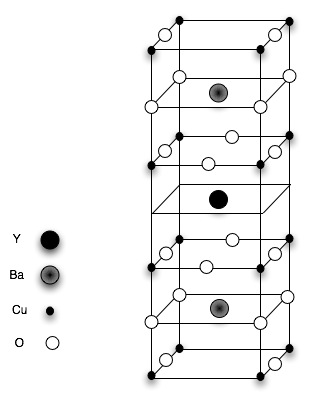
\includegraphics[scale=0.8]{YBCO}
\caption{Unit-cell structure of YBaCuO superconductor\cite{sheahen}}
\label{default}
\end{center}
\end{figure}

Ceramic superconductors like YBCO are often very anisotropic, that is, they have different properties in different crystalline directions. The superconducting current flows entirely in the planes of copper oxide in the crystal. YBCO has been found to be superconducting up to 92 K. This is important because then liquid helium is not required to cool the material, liquid nitrogen will suffice, which is much cheaper.
\subsection{Meissner effect}

The Meissner effect is the name given to the phenomenon in which a superconducting material, when cooled through T$_{c}$ expels any applied magnetic field inside it, up to a certain field strength known as the critical magnetic field $H_{c}(T)$. A field greater than this will overcome the Meissner effect and the material ceases to superconduct (it resumes superconduction once the field is removed). In any material, the applied magnetic field \textbf{H} and the magnetization \textbf{M} are related as follows:
\begin{equation}
\mathbf{B}=\mu_{0}(\mathbf{H+M})
\end{equation}
In a perfect diamagnet such as a superconductor, $\mathbf{M=-H}$, and \textbf{B}=0 as a result. The Meissner effect can be explained using the theory proposed by F. and H. London in 1935\cite{london}. The London equation is as follows:
\begin{equation}
\mathbf{j}=-\frac{1}{\mu_{0}\lambda_{L}^{2}}\mathbf{A}
\end{equation}
where \textbf{j} is the current density, and \textbf{A} is the magnetic vector potential, related to magnetic field \textbf{B} as follows:
\begin{equation}
\mathbf{B}=\nabla\times\mathbf{A}
\end{equation}
In the London gauge, $\nabla\cdot\mathbf{A}=0$. We take the curl of both sides of (2) to get:
\begin{equation}
\nabla\times\mathbf{j}=\frac{-1}{\mu_{0}\lambda_{L}^{2}}\mathbf{B}
\end{equation}
We know the Maxwell equation:
\begin{equation}
\nabla\times\mathbf{B}=\mu_{0}\mathbf{j}
\end{equation}
Taking the curl of both sides, we have:
\begin{equation}
\nabla\times\nabla\times\mathbf{B}=\mu_{0}\nabla\times\mathbf{j}
\end{equation}
Another Maxwell's equation gives us the divergence of \textbf{B}:
\begin{equation}
\nabla\cdot\mathbf{B}=0
\end{equation}
Therefore, (6) reduces to
\begin{equation}
-\nabla^{2}\mathbf{B}=\mu_{0}\nabla\times\mathbf{j}
\end{equation}
Combining this with (4), we obtain, for a superconductor:
\begin{equation}
\nabla^{2}\mathbf{B}=\frac{\mathbf{B}}{\lambda_{L}^{2}}
\end{equation}
This equation implies that a uniform magnetic field cannot exist within a superconductor.\cite{sheahen},\cite{kittel}. From the above equation, $\mathbf{B}=B_{0}e^{\frac{-z}{\lambda_{L}}}$, where $z$ is the distance from the surface to the point inside the semiconductor where the magnetic field is being measured. Thus we see that the magnetic field within a superconductor is expelled. $\lambda_{L}$is the London penetration depth, which indicates the depth of penetration of the magnetic field through the surface of the superconductor.

\section{Experimental Setup}
\subsection{Fabrication}
The method we used for fabricating our superconductor sample is adapted from the procedure laid out by Colin Greaves in ``Structural, Electrical and Magnetic Properties of Perovskite Ceramics"\cite{greaves}. The reagents used were dried Y$_{2}$O$_{3}$, CuO, and BaCO$_{3}$. The reagents were weighed out to give a Y:Ba:Cu ratio of 1:2:3, then ground together with a mortar and pestle until no white streaks were observable on grinding. The mixture was loaded into a circular die with a radius of approximately one inch, and then pressed at 5000 Kg in a hydraulic press to form a pellet approximately 3 mm in thickness. The pellet was then placed in a furnace programmed with the following sequence:

1. Heat to 930$^{o}$C and hold for 12 hours

2. Cool to 500$^{o}$C and hold for 1 hour

3. Cool to 400$^{o}$C at 50$^{o}$C h$^{-1}$

4. Cool to room temperature.

Once the furnace temperature was below 400$^{o}$C, the sample was removed from from the furnace and cooled. The sample, which was previously gray and shimmery and brittle, turned black and hard upon this treatment. To test whether our sample did in fact superconduct, we took it to a magnetic rail after cooling it in liquid nitrogen, and tested whether it levitated above the magnets due to the Meissner effect. It did in fact levitate (though not very high, due to its large size), so we concluded that we were successful in fabricating the YBa$_{2}$Cu$_{3}$O$_{7}$ ceramic superconductor.
\subsection{Characterization}
After fabrication, we proceeded to characterize the superconductor, that is, observe how its resistance changed with change in temperature. To do this, we adapted the simple procedure laid out by L. M. Le\'{o}n-Rossano\cite{leon}. A `T' type copper-constantan thermocouple was attached to the bottom of the sample with adhesive. The sample was placed in a metal sample holder, whose insides we covered with duct tape to provide insulation. Electric leads were then attached to the sample in the manner shown figure 2, with thin copper wires.
\begin{figure}[htbp]
\begin{center}
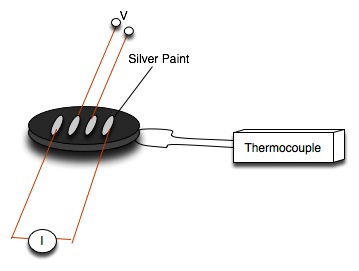
\includegraphics[scale=0.55]{superconductor.jpg}
\caption{Sample setup.}
\label{default}
\end{center}
\end{figure}
The sample in the sample holder was then lowered into a wide-based cylindrical styrofoam container. The leads from the thermocouple, and the two middle leads on the sample were connected to multimeters, and the two outer leads were connected to a constant current source of 0.3 A. We constructed a LabVIEW program to measure the multimeter readings from both multimeters simultaneously, convert the thermocouple multimeter voltage reading into a linearized temperature value, and then input a 2D array of these values into a spreadsheet. The last step in our experimental setup/procedure was to pour liquid nitrogen into the container, and then place a styrofoam lid on it, to slow down the temperature increase rate of the sample (so that we could take more data). The data obtained is presented in the next section.
\begin{figure}[htbp]
\begin{center}
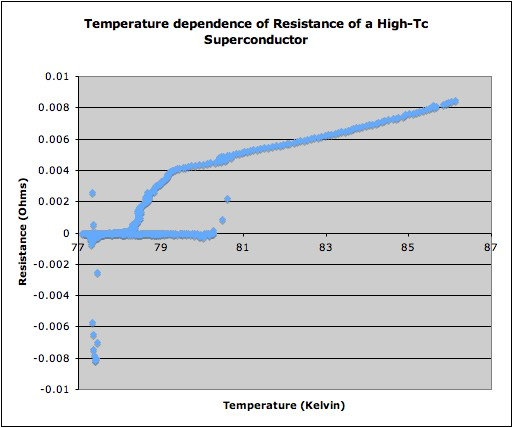
\includegraphics[scale=0.5]{superconductorgraph.jpg}
\caption{Plot of resistance of YBa$_{2}$Cu$_{3}$O$_{7}$ versus temperature. We see that there is a drastic drop in resistance once the temperature reaches 79 K, with it reaching zero at T$_{c}=78$K} 
\label{default}
\end{center}
\end{figure}
\section{Results and Analysis}
Figure 3 gives a plot of the change in resistance of the superconductor with temperature. From the graph we can observe that above approximately 79.4 K, there is a linear dependence of resistance on temperature. However, there is a drastic drop in resistance below this temperature, signifying a phase transition to superconductivity. At approximately 78.3 K, the resistance of the sample drops to zero. There are some spurious data points on the graph. These were caused by the leads becoming detached from the sample (they were notoriously tough to affix). These points appear as a horizontal line segment along the x-axis from 77 K to 80 K, and other outliers on the left hand side of the graph, and should be ignored. The critical temperature of ~78.3 K is well below the ideal T$_{c}$ of 93 K. This can be attributed to insufficient oxygen content\cite{greaves}, or crystal impurities and defects.

\section{Conclusion}
We successfully fabricated and characterized a high temperature YBa$_{2}$Cu$_{3}$O$_{7}$ ceramic superconductor sample. Further care and caution while preparing the sample will result in a higher T$_{c}$, closer to 93 K. Superconductors already have application in industry and in hospitals where they are used in the electromagnets for magnetic resonance imaging. High temperature superconductors would further reduce the refrigeration costs associated with normal superconductors. However, one as-yet unsurmounted practical setback is that it is extremely difficult to fashion ceramic superconductors into wires.\cite{sheahen}
% If in two-column mode, this environment will change to single-column
% format so that long equations can be displayed. Use
% sparingly.
%\begin{widetext}
% put long equation here
%\end{widetext}

% figures should be put into the text as floats.
% Use the graphics or graphicx packages (distributed with LaTeX2e)
% and the \includegraphics macro defined in those packages.
% See the LaTeX Graphics Companion by Michel Goosens, Sebastian Rahtz,
% and Frank Mittelbach for instance.
%
% Here is an example of the general form of a figure:
% Fill in the caption in the braces of the \caption{} command. Put the label
% that you will use with \ref{} command in the braces of the \label{} command.
% Use the figure* environment if the figure should span across the
% entire page. There is no need to do explicit centering.

% \begin{figure}
% \includegraphics{}%
% \caption{\label{}}
% \end{figure}

% Surround figure environment with turnpage environment for landscape
% figure
% \begin{turnpage}
% \begin{figure}
% \includegraphics{}%
% \caption{\label{}}
% \end{figure}
% \end{turnpage}

% tables should appear as floats within the text
%
% Here is an example of the general form of a table:
% Fill in the caption in the braces of the \caption{} command. Put the label
% that you will use with \ref{} command in the braces of the \label{} command.
% Insert the column specifiers (l, r, c, d, etc.) in the empty braces of the
% \begin{tabular}{} command.
% The ruledtabular enviroment adds doubled rules to table and sets a
% reasonable default table settings.
% Use the table* environment to get a full-width table in two-column
% Add \usepackage{longtable} and the longtable (or longtable*}
% environment for nicely formatted long tables. Or use the the [H]
% placement option to break a long table (with less control than 
% in longtable).
% \begin{table}%[H] add [H] placement to break table across pages
% \caption{\label{}}
% \begin{ruledtabular}
% \begin{tabular}{}
% Lines of table here ending with \\
% \end{tabular}
% \end{ruledtabular}
% \end{table}

% Surround table environment with turnpage environment for landscape
% table
% \begin{turnpage}
% \begin{table}
% \caption{\label{}}
% \begin{ruledtabular}
% \begin{tabular}{}
% \end{tabular}
% \end{ruledtabular}
% \end{table}
% \end{turnpage}

% Specify following sections are appendices. Use \appendix* if there
% only one appendix.
%\appendix
%\section{}

% If you have acknowledgments, this puts in the proper section head.
%\begin{acknowledgments}
% put your acknowledgments here.
%\end{acknowledgments}

% Create the reference section using BibTeX:
%\bibliography{basename of .bib file}
\begin{thebibliography}{9}
\bibitem{rose}
A. C. Rose-Innes and E.H. Rhoderick, \emph{Introduction to Superconductivity} (Pergamon Press Inc. New York, 1978), 2nd ed., pp 3-5.
\bibitem{onnes}
H. K. Onnes, Proceedings of the Koninklijke Akademie Van Wetenschappen Te Amsterdam \textbf{14}, 113 (1911).
 \bibitem{tinkman}
 M. Tinkman, \emph{Introduction to Superconductivity} (McGraw-Hill, Inc. New York 1996) pp. 1-16
 \bibitem{bednorz}
 J. G. Bednorz and K. M\"{u}ller, "Possible High T$_{c}$ Superconductivity in the Ba-La-Cu-O System," Z. Phys. B \textbf{64}, 189-193 (1986)
\bibitem{bcs}
Bardeen, J., Cooper, L. N., and Schrieffer, J. R., 
Theory of Superconductivity", \emph{Phys. Rev.} \textbf{108}, 1175 (1957)
\bibitem{sheahen}
T. P. Sheahen, \emph{Introduction to High-Temperature Superconductivity} (Plenum Press, New York, 1994) pp. 5,20
\bibitem{london}
F. and H. London, \emph{Proc. Royal Soc. A} \textbf{149}, 71 (1935)
\bibitem{kittel}
C. Kittel, \emph{Introduction to Solid State Physics} (Wiley India, New Delhi, 2004) 7th ed. pp 350-352
\bibitem{greaves}
C. Greaves, ``Structural, Electric and Magnetic Properties of Perovskite Ceramics", in \emph{Inorganic Experiments}, edited by J. Derek Woollins (VCH Verlagsgesellschaft mbH, Weinheim, 1994) pp. 265-270
\bibitem{leon}
L. M. Le\'{o}n, "An inexpensive and easy experiment to measure the electrical resistance
of high-T$_{c}$ superconductors as a function of temperature" Am. J. Phys. \textbf{65} 1024-1026 (1997)


\end{thebibliography}


\end{document}
%
% ****** End of file template.aps ******

